\documentclass[conference]{IEEEtran}
\IEEEoverridecommandlockouts
\usepackage[nocompress]{cite}
\usepackage{amsmath,amssymb,amsfonts}
\usepackage{graphicx}
\usepackage{textcomp}
\usepackage[T1,T2A]{fontenc}
\usepackage{booktabs}
\usepackage{multirow}
\usepackage{url}
\usepackage[none]{hyphenat}
\usepackage[utf8]{inputenc}
\usepackage[english,russian]{babel}

% Per EDM-2026 checklist: use "Keywords" rather than "Index Terms".
\renewcommand{\IEEEkeywordsname}{Ключевые слова}

% Plain (non-hyperlinked) URL formatting.
\urlstyle{tt}

\begin{document}

\title{Профилирование конвейера обработки МРТ головного мозга для проектирования мультиагентной системы}

\author{
\IEEEauthorblockN{Екатерина И. Ропперт}
\IEEEauthorblockA{Центр исследований в области\\
искусственного интеллекта\\
Новосибирский государственный университет\\
Новосибирск, Россия\\
e.roppert@g.nsu.ru}
\and
\IEEEauthorblockN{Баир Н. Тучинов}
\IEEEauthorblockA{Центр исследований в области\\
искусственного интеллекта\\
Новосибирский государственный университет\\
Новосибирск, Россия\\
bairt@nsu.ru}
\and
\IEEEauthorblockN{Евгений Н. Павловский}
\IEEEauthorblockA{Центр исследований в области\\
искусственного интеллекта\\
Новосибирский государственный университет\\
Новосибирск, Россия\\
e.pavlovskiy@g.nsu.ru}
}

\maketitle

\begin{abstract}
Автоматизированная обработка МРТ головного мозга для сегментации патологических очагов требует многоэтапного вычислительного конвейера с гетерогенными требованиями к ресурсам~--- от операций ввода-вывода при организации данных до CPU-интенсивной предобработки и GPU-ускоренного вывода нейронных сетей. Стратегии статического распределения ресурсов не позволяют эффективно справляться с этой гетерогенностью, поскольку каждый этап достигает насыщения при различном уровне параллелизма. В данной работе представлено систематическое профилирование производительности шестиэтапного конвейера обработки МРТ головного мозга с использованием набора данных UPENN-GBM по глиобластомам (100 пациентов, 110 сеансов) с контролируемой методологией бенчмаркинга, включающей очистку кэша. Выявлены точки насыщения, специфичные для каждого этапа: от 6 до 12 параллельных процессов для CPU-этапов и близкое к линейному масштабирование для двух GPU при сегментации. На основании полученных эмпирических профилей предложена архитектура мультиагентной системы, в которой агенты на основе модели <<Убеждения--Желания--Намерения>> (BDI) управляют отдельными этапами конвейера и согласовывают распределение ресурсов посредством протокола, вдохновлённого Contract Net, используя измеренные профили насыщения в качестве операционных знаний. Имитационное моделирование, сравнивающее четыре стратегии распределения~--- последовательную, поэтапно-последовательную параллельную, конвейерно-параллельную и мультиагентную с динамическим перераспределением~--- показывает, что мультиагентный подход обеспечивает ускорение в $4{,}7$ раза по сравнению с последовательной обработкой и сокращает общее время выполнения на 31\% по сравнению со статическим конвейерным параллелизмом для пакета из 100 пациентов, при этом средняя загрузка CPU возрастает с 12,6\% до 31,6\%.
\end{abstract}

\begin{IEEEkeywords}
мультиагентные системы, МРТ головного мозга, конвейер обработки изображений, профилирование производительности, распределение ресурсов, nnU-Net, параллельные вычисления
\end{IEEEkeywords}

\section{Введение}

Автоматизированный анализ магнитно-резонансной томографии (МРТ) головного мозга для сегментации патологических очагов требует сложного вычислительного конвейера, включающего множество гетерогенных этапов: организацию данных, конвертацию форматов, оценку качества, предобработку и вывод нейронных сетей~\cite{isensee2021}. Каждый этап обладает принципиально различными вычислительными характеристиками~--- от операций ввода-вывода файловой системы до CPU-интенсивной регистрации изображений и GPU-ускоренного глубокого обучения~--- что порождает сложную задачу управления ресурсами.

Стандартный подход к ускорению таких конвейеров~--- статическое распараллеливание, при котором фиксированное число параллельных процессов назначается одинаково для всех этапов. Однако эта стратегия неявно предполагает, что все этапы масштабируются одинаково с увеличением параллелизма, что на практике встречается редко. Когда отдельные этапы достигают своих точек насыщения при различных уровнях параллелизма, статически выделенные ресурсы простаивают, что приводит к низкой общей загрузке.

Мультиагентные системы (МАС) предлагают принципиальную альтернативу статическому распределению ресурсов. В МАС автономные агенты управляют отдельными этапами конвейера и динамически согласовывают распределение ресурсов на основе условий выполнения~\cite{wooldridge2009}. В отличие от простых параллельных планировщиков, агенты МАС обладают ключевыми свойствами, определёнными Вулдриджем и Дженнингсом~\cite{wooldridge1995}~--- автономностью, реактивностью, проактивностью и социальной способностью~--- что позволяет им адаптироваться к флуктуациям рабочей нагрузки и неоднородности оборудования без ручной перенастройки.

Последние достижения в области МАС на основе больших языковых моделей (LLM) для медицинской диагностики~\cite{tang2024,kim2024} продемонстрировали эффективность мультиагентной кооперации для сложных клинических задач, требующих декомпозиции и интеграции инструментов. Бенчмарковые исследования~\cite{zhu2025} подтверждают, что МАС превосходят одномодельные подходы именно тогда, когда задачи поддаются декомпозиции и требуют использования гетерогенных инструментов~--- условия, непосредственно выполняемые многоэтапными конвейерами обработки изображений.

Однако существует критический пробел: хотя архитектуры МАС всё активнее применяются для диагностического вывода, их использование для управления вычислительными ресурсами в конвейерах медицинской визуализации остаётся неисследованным. Проектирование эффективной МАС для оркестрации конвейера требует эмпирических знаний о поведении каждого этапа при распараллеливании~--- знаний, которые в настоящее время отсутствуют в литературе. В отличие от предшествующих работ по динамическому планированию, рассматривающих распределение ресурсов как задачу системной оптимизации, наш подход явным образом связывает эмпирическое профилирование производительности с агентно-ориентированным проектированием, кодируя измеренные профили насыщения непосредственно как убеждения BDI-агентов~--- методологический вклад, отсутствующий как в литературе по параллельным вычислениям, так и в литературе по МАС. Мы восполняем этот пробел посредством трёх вкладов: (1)~систематическое профилирование производительности шестиэтапного конвейера обработки МРТ головного мозга с контролируемой методологией очистки кэша, (2)~выявление точек насыщения, специфичных для каждого этапа, и распределения <<узких мест>>, а также (3)~обоснованное эмпирическими данными архитектурное предложение МАС, использующей эти профили в качестве базы знаний для динамического распределения ресурсов.

\section{Обзор литературы}

\subsection{Параллельная обработка в медицинской визуализации}

GPU-ускорение широко исследовано для обработки медицинских изображений. Kirimtat и Krejcar~\cite{kirimtat2024} рассматривают методы GPU-распараллеливания для анализа МРТ головного мозга, сообщая об ускорении в 7--90 раз для задач сегментации. Hashisho и др.~\cite{hashisho2024} классифицируют три типа параллелизма, применимых к конвейерам обработки изображений: параллелизм данных, задач и конвейерный параллелизм, определяя накладные расходы на обмен данными как ключевое <<узкое место>>. Фреймворк FAST~\cite{smistad2019} предоставляет унифицированный интерфейс для гетерогенного вывода на CPU, GPU и тензорных процессорах (TPU) для потоковой обработки медицинских изображений.

Для сегментации всего мозга Predescu и др.~\cite{predescu2024} оптимизируют пропускную способность конвейера SLANT на суперкомпьютере Summit, демонстрируя, что загрузка одного GPU падает ниже 25\% при обработке отдельных томов МРТ. Их метод перекрывающегося планирования фрагментов обеспечивает ускорение в $3{,}5$ раза на одном GPU с близким к линейному масштабированием на 96~GPU. Однако их оптимизация направлена только на этап глубокого обучения, при этом явно отмечается, что предобработка <<крайне нестабильна>>, но не исследуется. \textbf{Ни одна из существующих работ не профилирует все этапы полного конвейера обработки изображений для характеристики индивидуального поведения масштабирования каждого из них.}

\subsection{Мультиагентные системы в медицинском ИИ}

МАС получили значительное распространение в медицинской диагностике, прежде всего благодаря кооперации агентов на основе LLM. MedAgents~\cite{tang2024} показывает, что ролевая мультиагентная дискуссия повышает точность ответов на медицинские вопросы на 10,7\% по сравнению с одной LLM. MDAgents~\cite{kim2024} вводит адаптивную оценку сложности, направляя простые случаи одному агенту, а сложные~--- мультидисциплинарным командам, достигая лучших результатов на 7 из 10 медицинских бенчмарков. Более поздние системы интегрируют визуальный и количественный анализ: MedAgent-Pro~\cite{wang2025} сочетает агентное рассуждение с инструментами сегментации и обеспечивает улучшение F1 на +34,5 для офтальмологической диагностики, а LungNoduleAgent~\cite{yang2026} объединяет агентов обнаружения, оценки и рассуждения для диагностики узлов лёгких.

Бенчмарк MedAgentBoard~\cite{zhu2025} даёт критически важное свидетельство: МАС превосходят традиционные методы именно для задач с высокой степенью декомпозируемости и потребностью в интеграции инструментов, но не показывают преимуществ для простых текстовых задач. Этот результат непосредственно подтверждает гипотезу о том, что многоэтапные конвейеры обработки изображений~--- с их естественной декомпозируемостью и гетерогенными вычислительными требованиями~--- хорошо подходят для оркестрации на основе МАС. Тем не менее существующие работы по МАС в медицине направлены на диагностическое рассуждение, а не на управление вычислительными ресурсами, оставляя неизученными эмпирические профили, необходимые для проектирования ресурсно-ориентированной МАС для конвейеров обработки изображений.

\section{Описание системы}

Предлагаемая система реализует шестиэтапный модульный конвейер для автоматизированной сегментации патологических очагов головного мозга по данным МРТ (рис.~\ref{fig:pipeline}). Каждый этап оперирует на уровне отдельного пациента, что позволяет независимо распараллеливать обработку между пациентами. Все этапы выполняют проверку согласованности входных и выходных данных; пропущенные случаи регистрируются для полной прослеживаемости. Параметры конвейера управляются через единую YAML-конфигурацию, позволяющую настраивать каждый этап без модификации кода.

\begin{figure}[t]
\centering
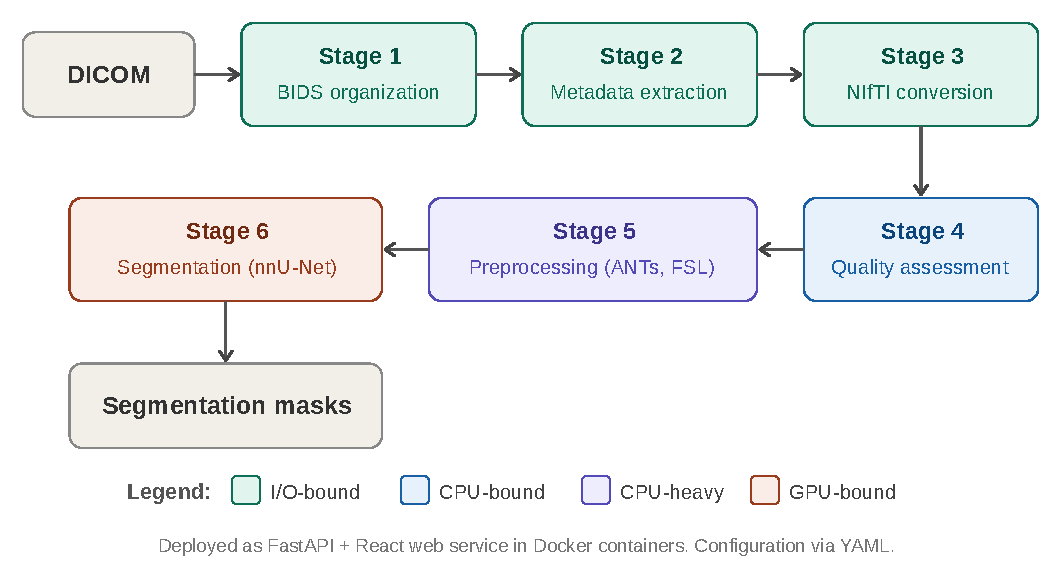
\includegraphics[width=\columnwidth]{fig1_pipeline_architecture.pdf}
\caption{Шестиэтапный конвейер обработки МРТ головного мозга. Цвета обозначают тип вычислительной нагрузки: зелёный = ввод-вывод, синий = CPU, фиолетовый = CPU-интенсивный, коралловый = GPU.}
\label{fig:pipeline}
\end{figure}

\textbf{Этап~1: Организация в формат BIDS.} Исходные файлы в формате Digital Imaging and Communications in Medicine (DICOM) с произвольной структурой каталогов реорганизуются в формат Brain Imaging Data Structure (BIDS)~\cite{gorgolewski2016}. Система автоматически определяет модальности МРТ (T1, T1ce, T2, FLAIR) и сопоставляет их с BIDS-совместимыми именами файлов. В данном исследовании входные данные включают 100 пациентов (110 сеансов визуализации, 424 серии МРТ, в каждом сеансе от 1 до 4 модальностей) из набора данных UPENN-GBM по глиобластомам~\cite{bakas2022}.

\textbf{Этап~2: Извлечение метаданных.} Выбранные теги DICOM извлекаются и сохраняются отдельно, после чего идентифицирующая информация пациента удаляется из исходных заголовков.

\textbf{Этап~3: Конвертация в NIfTI.} Серии DICOM конвертируются в формат Neuroimaging Informatics Technology Initiative (NIfTI) с помощью утилиты dcm2niix~\cite{li2016}.

\textbf{Этап~4: Оценка качества.} Для каждого тома вычисляются восемь метрик качества изображений: отношение сигнал/шум (SNR), отношение контраст/шум (CNR), критерий фокуса энтропии (EFC), отношение энергии переднего плана к фону (FBER), резкость градиента, анизотропия вокселей, дисперсия интенсивности и коэффициент вариации. Значения нормализуются и классифицируются по трём уровням качества~--- низкое, приемлемое, хорошее~--- на основе настраиваемых пороговых значений для каждой модальности.

\textbf{Этап~5: Предобработка.} Наиболее вычислительно затратный этап выполняет четыре последовательные операции: (1)~N4-коррекция неоднородности поля, (2)~аффинная регистрация опорной модальности (T1 по умолчанию) к стандартному атласу мозга с помощью Advanced Normalization Tools (ANTs)~\cite{avants2009}, с последующей регистрацией остальных модальностей к совмещённому опорному изображению, (3)~удаление черепа с помощью FSL Brain Extraction Tool (BET)~\cite{smith2002} и (4)~нормализация интенсивности.

\textbf{Этап~6: Сегментация.} Сегментация патологических очагов головного мозга выполняется с помощью nnU-Net~\cite{isensee2021}, выбранной благодаря самонастраивающейся архитектуре и подтверждённой эффективности на бенчмарках опухолей головного мозга. Модель предобучена на многоклассовом наборе данных по опухолям мозга~\cite{pnev2022}. Вывод выполняется на настраиваемом GPU-сервере с поддержкой параллелизации на нескольких GPU посредством асинхронной клиентской архитектуры с явным назначением устройств CUDA. Архитектура конвейера не зависит от модели: бэкенд сегментации может быть заменён без воздействия на другие этапы.

Конвейер развёрнут как веб-сервис с бэкендом на FastAPI и фронтендом на React, контейнеризованный с помощью Docker. Исходный код и скрипты бенчмаркинга доступны в открытом репозитории проекта \texttt{KateRoppert/mri\_ai\_service} на GitHub.

\section{Экспериментальные результаты}

\subsection{Экспериментальная установка}

Все эксперименты с CPU-нагрузкой (этапы~1--5) проводились на рабочей станции с процессором Intel Core i7-13700KF (16 ядер / 24 потока, до 5,4~ГГц), 64~ГБ DDR5 RAM, NVMe SSD, под управлением Ubuntu 24.04 LTS. Для GPU-сегментации (этап~6) использовались три сервера: \textit{Сервер~A} (2$\times$NVIDIA RTX A4500, 20~ГБ VRAM каждый), \textit{Сервер~B} (1$\times$NVIDIA Quadro RTX 8000, 48~ГБ VRAM) и \textit{Сервер~C} (1$\times$NVIDIA GeForce GTX TITAN X, 12~ГБ VRAM).

Набор данных включает 100 пациентов из коллекции UPENN-GBM~\cite{bakas2022}, что составляет 110 сеансов визуализации по четырём модальностям МРТ (T1, T1ce, T2, FLAIR). Не все сеансы содержат полный набор модальностей: 103 сеанса включают опорную модальность T1, необходимую для предобработки (этап~5), а 98 сеансов содержат все четыре модальности, требуемые моделью nnU-Net для сегментации (этап~6). Для каждого CPU-этапа число параллельных процессов варьировалось от 1 до 20.

\subsection{Методология}

Для обеспечения валидности измерений был реализован контролируемый протокол бенчмаркинга. Перед каждым запуском эксперимента дисковый кэш операционной системы явно очищался (команда \texttt{sync} с последующей \texttt{echo 3 > /proc/sys/vm/drop\_caches}) с 2-секундной паузой стабилизации. Этот шаг оказался критически важным: предварительные эксперименты без очистки кэша демонстрировали искусственно завышенные ускорения для этапов, ограниченных вводом-выводом, причём некоторые конфигурации казались в 2--4 раза быстрее реальной скорости из-за кэшированного чтения файлов. Где это было вычислительно целесообразно, каждая конфигурация выполнялась дважды, и результаты усреднялись. Этапы~1--3 показали разброс менее 10\% по всем конфигурациям; этапы~4--5 выполнялись однократно ввиду длительного времени выполнения (2+ часа на конфигурацию).

\subsection{Результаты распараллеливания}

В таблице~\ref{tab:optimal} приведены оптимальные конфигурации для каждого этапа, а на рис.~\ref{fig:speedup} представлены кривые ускорения. Результаты выявляют выраженную гетерогенность масштабирования по этапам.

\begin{table}[t]
\centering
\caption{Оптимальные конфигурации параллелизма для каждого этапа. Время и ускорение указаны в точке насыщения (Нас.), определяемой как минимальное число процессов, после которого прирост пропускной способности составляет менее 5\%.}
\label{tab:optimal}
\begin{tabular}{clccccc}
\toprule
Этап & Название & Тип & Сеан. & Нас. & Время(с) & Уск. \\
\midrule
1 & Орг. BIDS & В/В & 110 & 8 & 188,6 & 3,49$\times$ \\
2 & Метаданные & В/В & 110 & 8 & 0,2 & 3,49$\times$ \\
3 & Конв. NIfTI & В/В+ & 110 & 8 & 35,5 & 3,79$\times$ \\
4 & Качество & CPU & 110 & 12 & 114,0 & 5,22$\times$ \\
5 & Предобр. & CPU & 103 & 6 & 1490,1 & 2,17$\times$ \\
6 & Сегмент. & GPU & 98 & 2GPU & 1230,3 & 1,94$\times$ \\
\bottomrule
\end{tabular}
\end{table}

\begin{figure}[t]
\centering
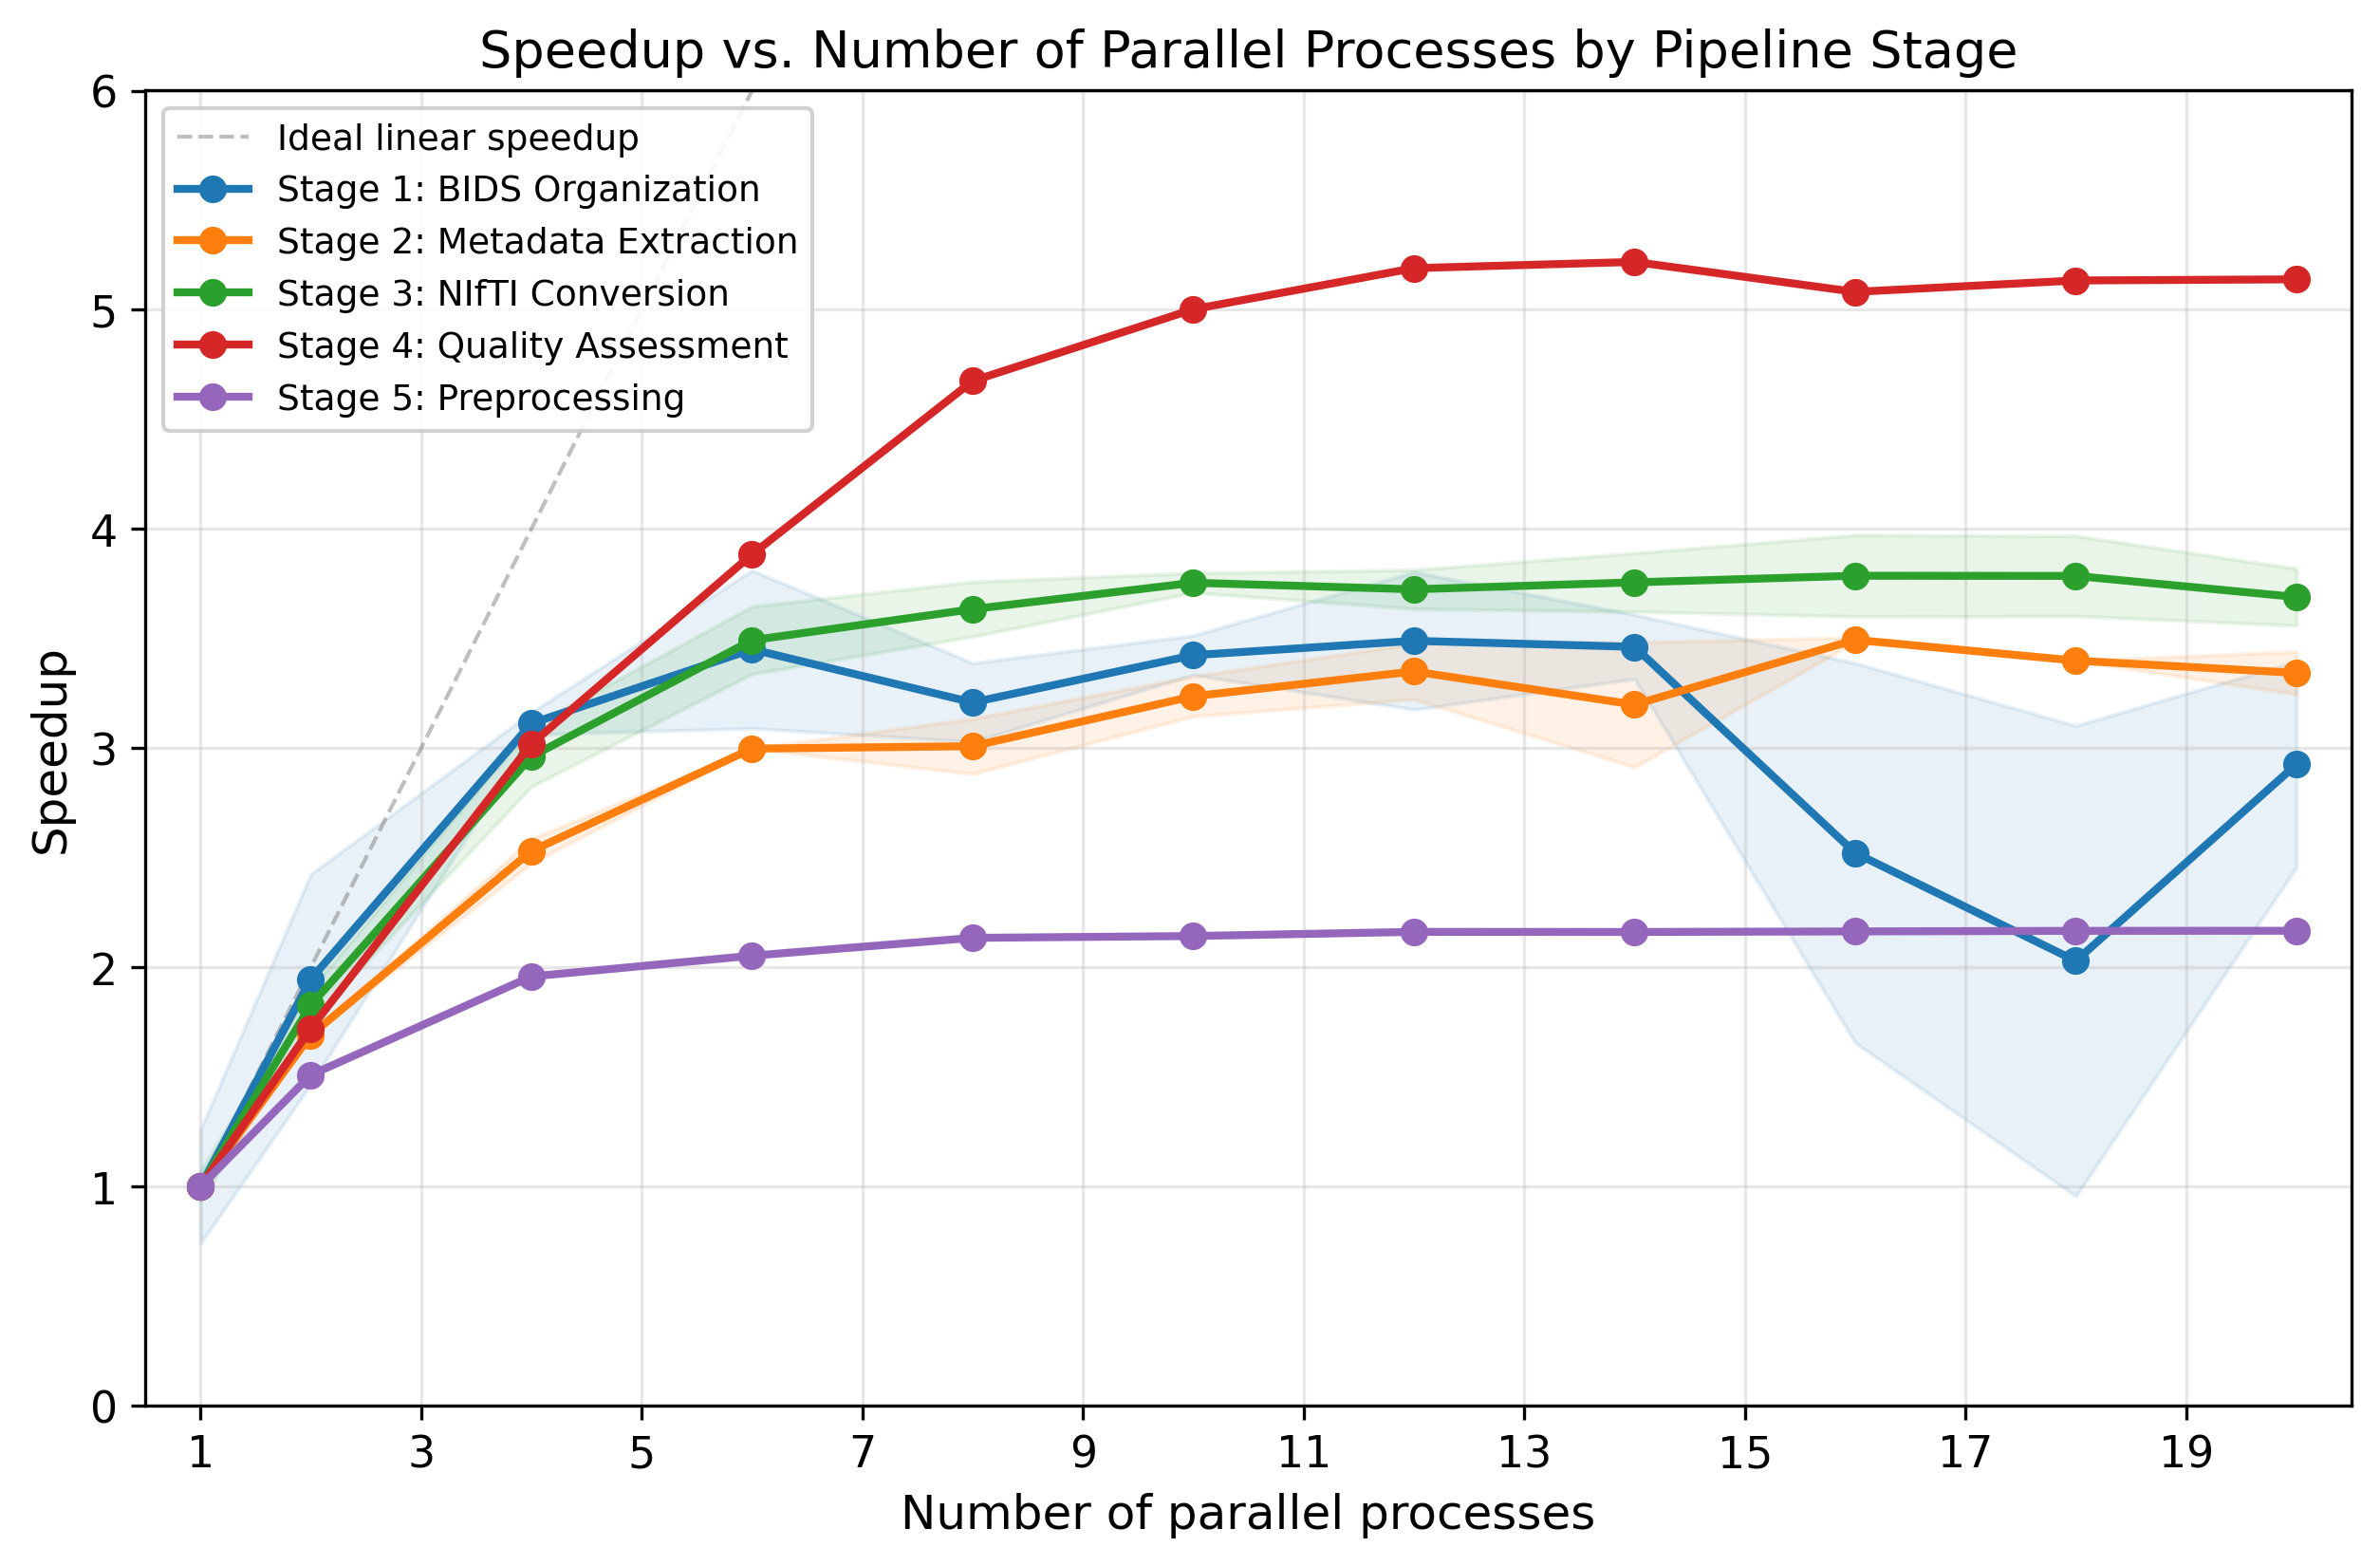
\includegraphics[width=\columnwidth]{speedup_all_stages.png}
\caption{Ускорение в зависимости от числа параллельных процессов по этапам конвейера. Закрашенные полосы обозначают разброс между двумя экспериментальными запусками. Штриховая линия~--- идеальное линейное ускорение.}
\label{fig:speedup}
\end{figure}

\textbf{Этапы~1--3 (ограничены вводом-выводом)} демонстрируют схожее насыщение при 6--8 процессах с ускорением в 3,5--3,8 раза. За этой точкой пропускная способность дискового ввода-вывода становится ограничивающим фактором. \textbf{Этап~4 (CPU-ограниченный)} показывает наилучшую масштабируемость, достигая ускорения в $5{,}22$ раза при 12 процессах с близким к линейному масштабированием до $w = 10$. \textbf{Этап~5 (CPU-интенсивный)} наиболее устойчив к распараллеливанию, насыщаясь уже при 6 процессах с ускорением лишь в $2{,}17$ раза. Каждый экземпляр предобработки внутренне использует множество потоков для регистрации ANTs и операций FSL, вызывая конкуренцию за ядра CPU. Профилирование памяти показало, что пиковое потребление RAM снизилось с 1,7~ГБ при $w=1$ до 338~МБ при $w \geq 2$, что указывает на то, что насыщение обусловлено конкуренцией за CPU, а не исчерпанием памяти. Этот этап потребляет 47,8\% общего времени конвейера, являясь основным <<узким местом>>. \textbf{Этап~6 (GPU-ограниченный)} профилирован на трёх конфигурациях серверов (табл.~\ref{tab:gpu}); двухпроцессорная GPU-конфигурация на \textit{Сервере~A} обеспечивает ускорение в $1{,}94$ раза при параллельной эффективности 96,8\%.

\begin{table}[t]
\centering
\caption{Производительность GPU-сегментации на различных серверах. \textit{Сервер~A} имеет 2 доступных GPU; остальные серверы~--- по 1~GPU.}
\label{tab:gpu}
\begin{tabular}{llccc}
\toprule
Сервер & GPU & Исп. & Время/сеан.(с) & Уск. \\
\midrule
Сервер~A & 2$\times$RTX A4500 & 1 & 24,31 & 1,00$\times$ \\
Сервер~A & 2$\times$RTX A4500 & 2 & 12,55 & 1,94$\times$ \\
Сервер~B & Quadro RTX 8000 & 1 & 56,43 & 1,00$\times$ \\
Сервер~C & GTX TITAN X & 1 & 128,85 & 1,00$\times$ \\
\bottomrule
\end{tabular}
\end{table}

\subsection{Анализ <<узких мест>>}

Два этапа доминируют в общем времени конвейера: предобработка (47,8\%) и сегментация (44,3\%), в совокупности составляя 92,1\%. Эти доли отражают время обработки одного сеанса при индивидуально оптимальной конфигурации каждого этапа и обозначают относительный вычислительный вес каждого этапа, а не одновременно достижимую рабочую точку. Два доминирующих этапа предъявляют принципиально различные требования к ресурсам: этап~5 ограничен CPU и оперативной памятью, тогда как этап~6 ограничен GPU. Эта взаимодополняемость означает, что они могут выполняться одновременно без конкуренции за ресурсы~--- наблюдение, мотивирующее архитектуру МАС, предложенную в разделе~V.

\section{Предлагаемая архитектура МАС}

Гетерогенные профили насыщения, выявленные в разделе~IV, демонстрируют, что ни одна статическая конфигурация не является оптимальной для всех этапов конвейера. В данном разделе предлагается архитектура МАС, использующая эмпирические профили производительности в качестве операционной базы знаний для динамического согласования ресурсов. Основной вклад данной работы~--- методология профилирования и её результаты; представленная архитектура является проектным предложением, основанным на устоявшейся теории МАС, с полной реализацией и валидацией в качестве будущей работы.

\subsection{Модель агента}

Каждый менеджер этапа моделируется как BDI-агент (<<Убеждения--Желания--Намерения>>)~\cite{wooldridge1995}. \textbf{Убеждения} кодируют операционное состояние агента: текущую глубину очереди, число активных процессов, наблюдаемую пропускную способность и эмпирически определённый профиль насыщения из табл.~\ref{tab:optimal}. \textbf{Желания} представляют цели агента: минимизация времени обработки очереди при избегании растраты ресурсов за пределами точки насыщения. \textbf{Намерения}~--- это принятые агентом решения: запросить дополнительные процессы, освободить избыточные процессы или сохранить текущее распределение.

\subsection{Обзор архитектуры}

Система состоит из трёх уровней. \textbf{Уровень~1: Агент-брокер} выступает в роли \textit{посредника}, а не центрального контроллера; он поддерживает глобальный пул ресурсов, обеспечивает согласование между менеджерами этапов и реализует системные ограничения. \textbf{Уровень~2: Агенты-менеджеры этапов} ($\times$6)~--- автономные BDI-агенты, которые независимо мониторят свои очереди, оценивают, улучшит ли выделение дополнительных ресурсов пропускную способность, и участвуют в согласовании ресурсов через протокол, вдохновлённый Contract Net. \textbf{Уровень~3: Рабочие процессы}~--- управляемые вычислительные ресурсы, выделяемые менеджерам этапов по результатам согласования. Архитектура удовлетворяет свойствам МАС по Вулдриджу и Дженнингсу~\cite{wooldridge1995}: автономность (менеджеры этапов принимают решения самостоятельно, брокер не может принудительно освободить ресурсы), реактивность (агенты реагируют на аномалии времени выполнения без внешнего вмешательства), проактивность (агенты предвосхищают спрос и освобождают ресурсы до того, как их попросят) и социальная способность (содержательная коммуникация через протокол согласования).

\subsection{Протокол согласования ресурсов}

Распределение ресурсов следует протоколу, вдохновлённому протоколом Contract Net (CNP)~\cite{smith1980}~--- фундаментальным механизмом координации в МАС, широко применяемым в современных агентных фреймворках~\cite{dorri2018}. \textit{Шаг~1: Объявление.} Когда очередь менеджера этапа превышает пороговое значение и число его процессов ниже точки насыщения, он отправляет запрос ресурсов брокеру. \textit{Шаг~2: Запрос предложений.} Брокер рассылает запрос; другие менеджеры этапов могут предложить освободить процессы, если их очередь пуста или текущее распределение превышает насыщение. \textit{Шаг~3: Оценка и назначение.} Брокер оценивает предложения и распределяет ресурсы, приоритизируя освобождение от наиболее перенасыщенных этапов. Данный протокол сохраняет автономию агентов: менеджеры этапов самостоятельно решают, \textit{подавать ли} предложение и \textit{сколько} процессов предложить.

\section{Моделирование производительности}

Для количественной оценки преимуществ динамического распределения ресурсов построена имитационная модель, управляемая эмпирическими данными о пропускной способности из раздела~IV. Модель сравнивает четыре стратегии при размерах пакетов 20, 50 и 100 пациентов, используя $P = 24$ процесса CPU и $G = 2$ устройства GPU.

\subsection{Модель пропускной способности}

Для каждого CPU-этапа $i$ с $w$ выделенными процессами пропускная способность рассчитывается на основе эмпирических измерений:
\begin{equation}
\theta(i, w) = N_i / T(i, w),
\end{equation}
где $N_i$~--- число сеансов в эксперименте, а $T(i, w)$~--- измеренное реальное время выполнения. Для промежуточных значений числа рабочих процессов применяется линейная интерполяция.

\subsection{Четыре стратегии распределения}

\textbf{Стратегия~1: Последовательная.} Один процесс, этапы выполняются один за другим: $M_{\text{seq}} = \sum n_i / \theta(i, 1)$.

\textbf{Стратегия~2: Поэтапно-последовательная параллельная.} Весь пул CPU выделяется каждому этапу, этапы выполняются последовательно (текущая система): $M_{\text{ss}} = \sum n_i / \theta(i, \min(P, s_i))$, где $s_i$ обозначает эмпирически определённую точку насыщения этапа~$i$ (столбец <<Нас.>> в табл.~\ref{tab:optimal}).

\textbf{Стратегия~3: Конвейерно-параллельная.} Этапы выполняются одновременно с фиксированным распределением $w_i$, масштабированным до бюджета $P$: $M_{\text{pip}} = \max_i \{ \text{start}(i) + n_i / \theta(i, w_i) \}$.

\textbf{Стратегия~4: МАС (динамическая).} Дискретно-событийное моделирование с начальным распределением как в стратегии~3, периодическим перераспределением каждые 10~с и накладными расходами 1~с на цикл перераспределения.

В стратегиях~3 и~4 GPU-сегментация работает как часть конвейера: она начинается, как только первый сеанс завершает предобработку, перекрываясь с продолжающимися CPU-этапами. Для 100 пациентов это устраняет примерно 25 минут простоя GPU, присутствующего в стратегиях~1 и~2.

\subsection{Результаты}

В таблице~\ref{tab:sim} представлены результаты моделирования, а на рис.~\ref{fig:makespan} визуализировано сравнение времени выполнения.

\begin{table}[t]
\centering
\caption{Результаты моделирования: четыре стратегии распределения}
\label{tab:sim}
\begin{tabular}{clcccc}
\toprule
$N$ & Стратегия & Время & Уск. & CPU\% & Прп \\
\midrule
\multirow{4}{*}{20}
& Последовательная & 21,4 & 1,00$\times$ & 4,2 & 56 \\
& Поэтапн.-посл. & 9,4 & 2,29$\times$ & 46,0 & 128 \\
& Конвейерная & 6,6 & 3,23$\times$ & 12,4 & 181 \\
& \textbf{МАС} & \textbf{5,4} & \textbf{4,00$\times$} & \textbf{29,4} & \textbf{224} \\
\midrule
\multirow{4}{*}{50}
& Последовательная & 53,3 & 1,00$\times$ & 4,2 & 56 \\
& Поэтапн.-посл. & 23,3 & 2,29$\times$ & 45,8 & 129 \\
& Конвейерная & 16,3 & 3,26$\times$ & 12,6 & 184 \\
& \textbf{МАС} & \textbf{10,9} & \textbf{4,88$\times$} & \textbf{31,9} & \textbf{274} \\
\midrule
\multirow{4}{*}{100}
& Последовательная & 106,2 & 1,00$\times$ & 4,2 & 57 \\
& Поэтапн.-посл. & 46,4 & 2,29$\times$ & 46,0 & 129 \\
& Конвейерная & 32,6 & 3,26$\times$ & 12,6 & 184 \\
& \textbf{МАС} & \textbf{22,6} & \textbf{4,7$\times$} & \textbf{31,6} & \textbf{266} \\
\bottomrule
\end{tabular}\\[4pt]
\footnotesize $N$ = размер пакета; Время = время выполнения (мин); Прп = пропускная способность (пац./ч).
\end{table}

\begin{figure}[t]
\centering
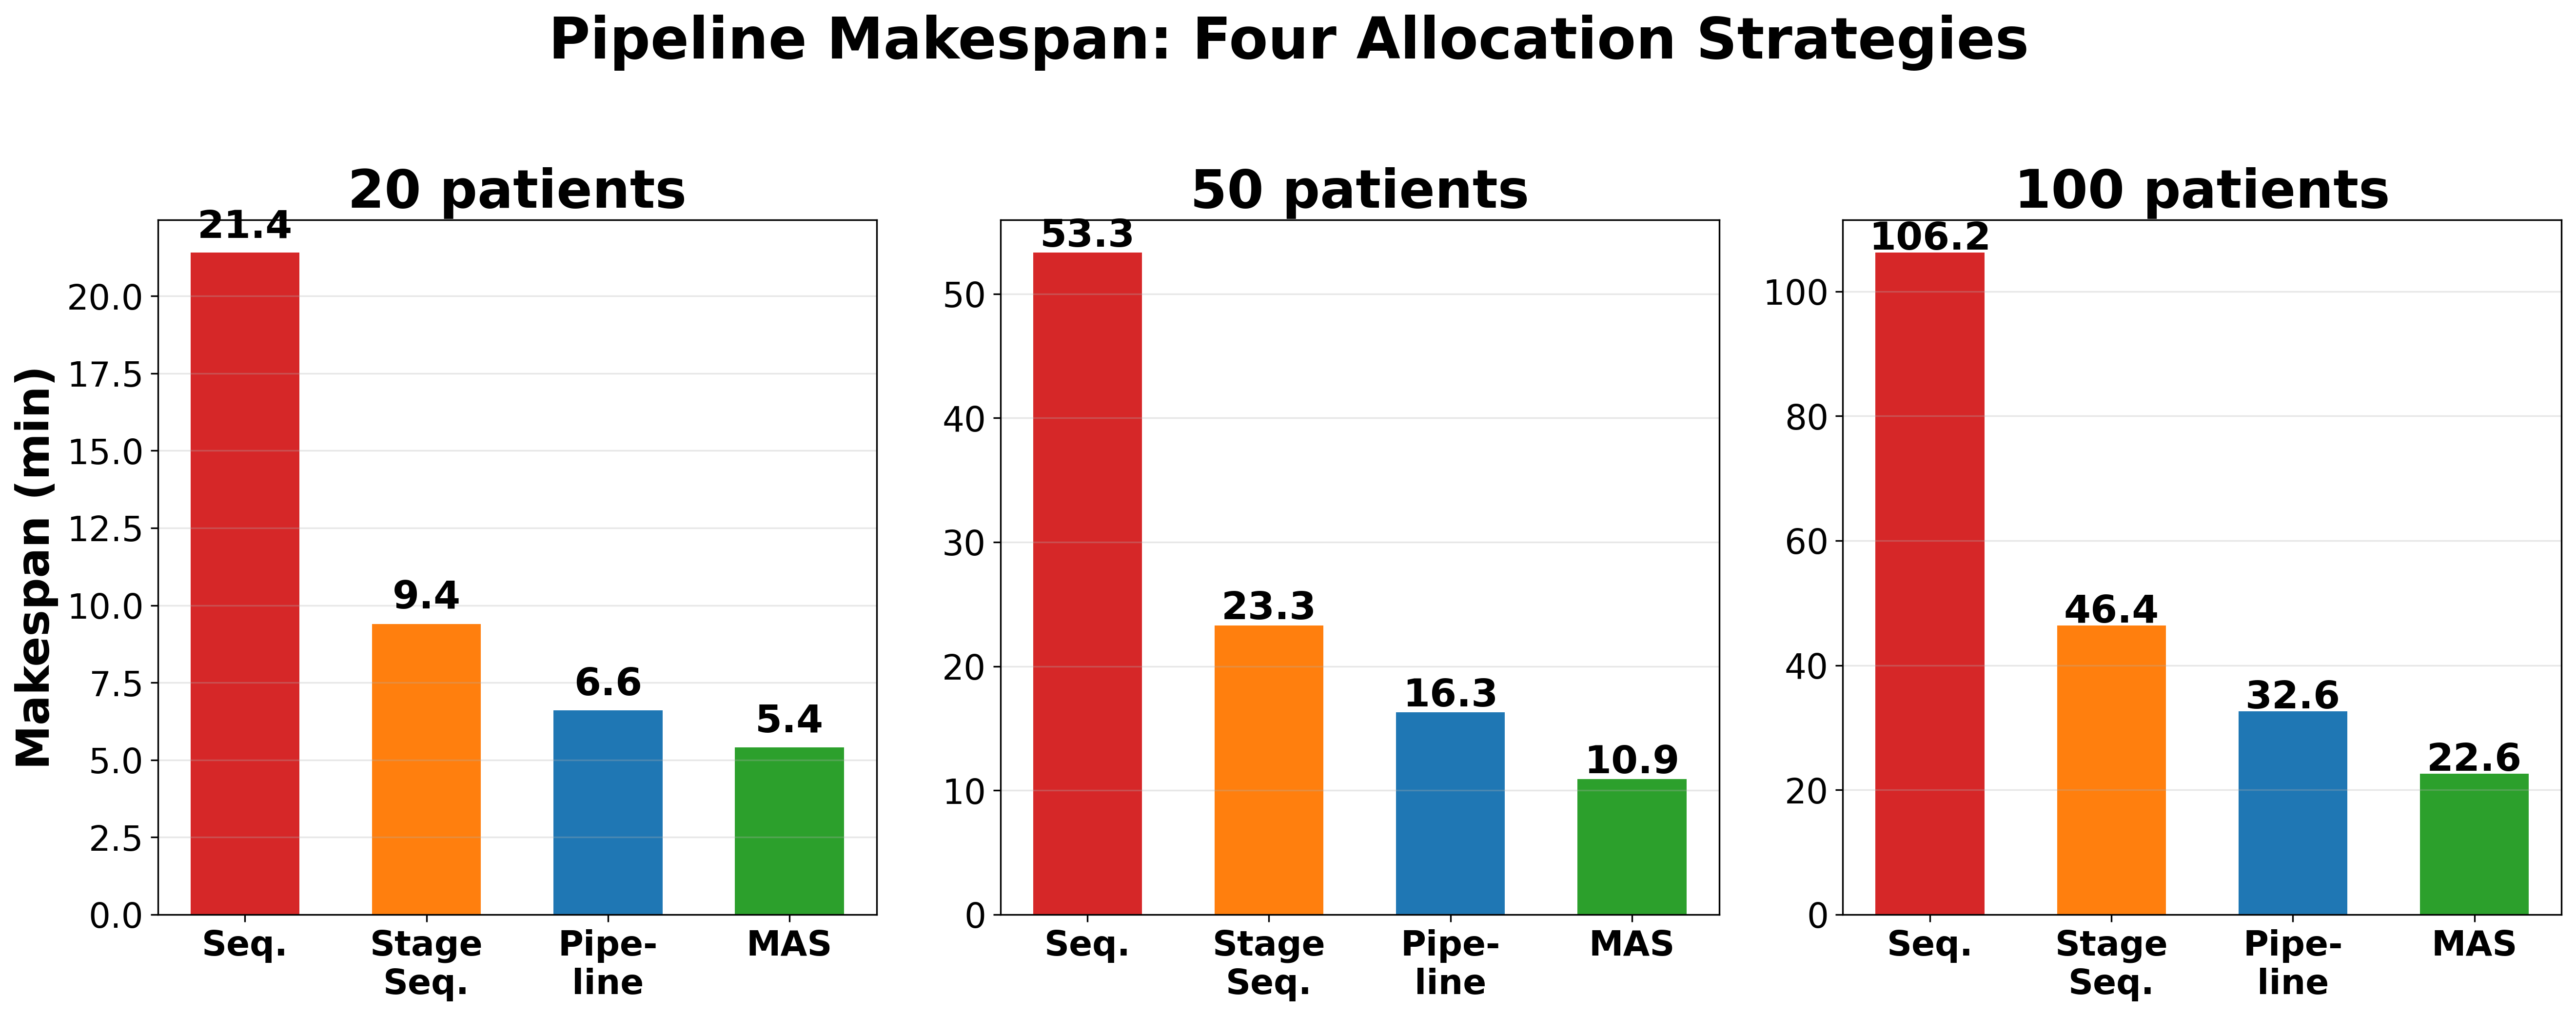
\includegraphics[width=\columnwidth]{makespan_comparison.png}
\caption{Сравнение времени выполнения конвейера для четырёх стратегий распределения ресурсов при размерах пакетов 20, 50 и 100 пациентов.}
\label{fig:makespan}
\end{figure}

Выявлены четыре ключевых результата. Во-первых, конвейерное перекрытие важнее глубины ресурсов на каждом этапе: конвейерно-параллельная стратегия обеспечивает ускорение в $3{,}26$ раза против $2{,}29$ раза для поэтапно-последовательной при 100 пациентах, несмотря на то что каждый этап получает меньше процессов. Во-вторых, динамическое перераспределение компенсирует разрыв в загрузке: МАС достигает ускорения в $4{,}7$ раза при 100 пациентах (улучшение на 44\% по сравнению с конвейерно-параллельной стратегией), поскольку процессы от завершённых ранних этапов мигрируют к <<узкому месту>>~--- предобработке, которая масштабируется от 2 до 6 рабочих процессов. В-третьих, выигрыш растёт с увеличением размера пакета: МАС сокращает время выполнения на 19\% по сравнению с конвейерной стратегией при 20 пациентах и на 31\% при 100. В-четвёртых, перекрытие GPU критически важно~--- в режиме МАС GPU-сегментация выполняется одновременно с предобработкой, и их пропускные способности почти совпадают (1 сеанс за 12,5~с vs 15~с), обеспечивая сбалансированный конвейер. Преимущество МАС устойчиво к накладным расходам на согласование: при 100 пациентах (${\sim}20$ циклов перераспределения) увеличение накладных расходов на цикл с 1~с до 10~с повышает время выполнения лишь с 22,6 до 25,6~мин, что всё ещё на 21\% быстрее конвейерно-параллельной стратегии.

\section{Обсуждение}

\subsection{МАС vs.\ параллелизм}

Полученные преимущества в принципе могут быть достигнуты динамическим планировщиком без мультиагентных концепций, а моделирование в разделе~VI оценивает эффект динамического перераспределения как принцип, а не специфические накладные расходы мультиагентного согласования. Тем не менее три архитектурных отличия обосновывают применение МАС: \textit{децентрализованное знание} (каждый менеджер этапа инкапсулирует собственный профиль насыщения как локальное убеждение, поэтому добавление нового этапа конвейера требует лишь развёртывания нового агента); \textit{согласование вместо диктата} (протокол на основе CNP позволяет агентам отклонять освобождение ресурсов на основании локального состояния, обрабатывая отклонения от эмпирической модели в реальном времени); и \textit{проактивное поведение} (агенты предвосхищают спрос и освобождают ресурсы до того, как их запрашивают, сокращая эффективную задержку перераспределения). Эти преимущества~--- децентрализованное управление знаниями, отказоустойчивость через автономию агентов и модульная расширяемость~--- становятся критически важными при многоузловом клиническом развёртывании, не охватываемом одномашинным моделированием.

Существующие кластерные планировщики, такие как YARN, Kubernetes и Slurm, оперируют на уровне контейнеров или узлов и распределяют ресурсы на основе декларированных требований, а не эмпирических профилей насыщения, специфичных для каждого этапа. Они не способны выразить ограничение <<Этап~5 не получает выигрыша свыше 6~процессов, тогда как Этап~4 масштабируется до~12>> без ручной настройки, которую необходимо обновлять при каждом изменении конвейера, оборудования или набора данных. Предлагаемая МАС интернализирует эти профили как убеждения агентов, обеспечивая автоматическую адаптацию~--- возможность, которой планировщики общего назначения лишены по своей архитектуре.

\subsection{Клиническая применимость}

Текущие клинические рабочие процессы обрабатывают исследования МРТ последовательно. Даже при оптимальном статическом распараллеливании обработка 100 исследований занимает 46 минут. Конвейер на основе МАС сокращает это время до 23 минут и выдаёт результаты инкрементально: согласно трассировке моделирования, первый результат сегментации становится доступен в течение нескольких минут после запуска конвейера, обеспечивая \textit{потоковый} клинический рабочий процесс. Методология профилирования универсальна: новая клиника может запустить скрипт бенчмаркинга, получить собственные профили насыщения и сконфигурировать агентов МАС соответствующим образом.

\subsection{Ограничения}

Архитектура МАС и модель производительности оценены только посредством моделирования, а не на развёрнутом прототипе; следовательно, реальные накладные расходы на коммуникацию и затраты на миграцию процессов ещё предстоит измерить. Моделирование предполагает детерминированную пропускную способность для каждого сеанса, выведенную из пакетных средних, тогда как реальные клинические данные демонстрируют вариабельность между пациентами по размеру изображений, разрешению и полноте модальностей, что может сдвинуть точки насыщения и повлиять на время перераспределения. Все эмпирические данные получены на наборе UPENN-GBM по глиобластомам с мультимодальной 3D~МРТ; профили насыщения могут существенно отличаться для других патологий (например, рассеянный склероз с меньшим объёмом очагов), одномодальных протоколов или наборов данных существенно иного размера. Накладные расходы на перераспределение в 1~секунду являются оптимистичной оценкой, а GPU-сегментация составляет ${\sim}80\%$ времени выполнения МАС~--- дальнейшее улучшение требует дополнительных GPU-ресурсов.

\section{Заключение}

В данной работе рассмотрена задача управления ресурсами в многоэтапных конвейерах обработки МРТ головного мозга посредством эмпирического профилирования, архитектурного проектирования и оценки на основе имитационного моделирования. Шестиэтапный конвейер был протестирован по контролируемому протоколу с очисткой кэша, что позволило выявить точки насыщения, специфичные для каждого этапа (6--12 процессов), и показать, что предобработка и сегментация занимают 92\% времени конвейера. Полученные эмпирические точки насыщения и кривые пропускной способности непосредственно служат убеждениями BDI-агентов, связывая системный бенчмаркинг и проектирование мультиагентной архитектуры, и обосновывают трёхуровневую МАС (брокер, менеджеры этапов, рабочие процессы) с согласованием по протоколу, вдохновлённому Contract Net. В моделировании МАС обеспечивает ускорение в $4{,}7$ раза по сравнению с последовательной обработкой при 100 пациентах, превосходя как поэтапно-последовательную ($2{,}29$ раза), так и конвейерно-параллельную ($3{,}26$ раза) стратегии; перекрытие GPU/CPU и динамическая миграция ресурсов являются основными механизмами, обеспечивающими преимущество. Дальнейшая работа будет развиваться в трёх направлениях. Во-первых, будет реализован прототип МАС с использованием агентного фреймворка SPADE в рамках существующей инфраструктуры FastAPI/Docker; ключевые метрики~--- задержка межагентных сообщений, время сходимости согласования и накладные расходы на миграцию процессов~--- позволят напрямую сравнить результаты моделирования и эмпирической МАС. Во-вторых, исследование профилирования будет воспроизведено на дополнительных наборах данных~--- включая MS60 для сегментации очагов рассеянного склероза~--- для оценки вариативности профилей насыщения при различных патологиях и протоколах визуализации. В-третьих, модель агентов будет расширена для поддержки многоузлового распределённого развёртывания с гетерогенными GPU-ресурсами между клиническими площадками, где преимущества децентрализации МАС перед централизованными планировщиками должны проявиться наиболее ярко.

\section*{Благодарности}

Работа выполнена при поддержке гранта для исследовательских центров, предоставленного Министерством экономического развития Российской Федерации в соответствии с соглашением о субсидии с Новосибирским государственным университетом от 17 апреля 2025~г. №~139-15-2025-006: ИГК 000000C313925P3S0002.

\begin{thebibliography}{20}
\bibitem{isensee2021} F. Isensee, P.~F. Jaeger, S.~A.~A. Kohl, J. Petersen, and K.~H. Maier-Hein, ``nnU-Net: a self-configuring method for deep learning-based biomedical image segmentation,'' \textit{Nature Methods}, vol.~18, no.~2, pp.~203--211, 2021, doi: 10.1038/s41592-020-01008-z.

\bibitem{wooldridge2009} M. Wooldridge, \textit{An Introduction to MultiAgent Systems}, 2nd~ed. Chichester, U.K.: Wiley, 2009, pp.~1--461, ISBN: 978-0-470-51946-2.

\bibitem{wooldridge1995} M. Wooldridge and N.~R. Jennings, ``Intelligent agents: Theory and practice,'' \textit{The Knowledge Engineering Review}, vol.~10, no.~2, pp.~115--152, 1995, doi: 10.1017/S0269888900008122.

\bibitem{tang2024} X. Tang, A. Zou, Z. Zhang, Z. Li, Y. Zhao, X. Zhang, A. Cohan, and M. Gerstein, ``MedAgents: Large language models as collaborators for zero-shot medical reasoning,'' in \textit{Findings of the Association for Computational Linguistics: ACL 2024}, Bangkok, Thailand, 2024, pp.~599--621, doi: 10.18653/v1/2024.findings-acl.33.

\bibitem{kim2024} Y. Kim, C. Park, H. Jeong, Y.~S. Chan, X. Xu, D. McDuff, H. Lee, M. Ghassemi, C. Breazeal, and H.~W. Park, ``MDAgents: An adaptive collaboration of LLMs for medical decision-making,'' in \textit{Advances in Neural Information Processing Systems 37 (NeurIPS 2024)}, Vancouver, Canada, 2024, pp.~1--26, doi: 10.48550/arXiv.2404.15155.

\bibitem{zhu2025} K. Zhu, Y. Yang, H. Wang, Z. Wu, J. Wang, and B. Xu, ``MedAgentBoard: Benchmarking multi-agent collaboration with conventional methods for diverse medical tasks,'' in \textit{Proc. 39th Conf. Neural Information Processing Systems (NeurIPS 2025) Datasets and Benchmarks Track}, 2025, pp.~1--32, doi: 10.48550/arXiv.2505.12371.

\bibitem{kirimtat2024} A. Kirimtat and O. Krejcar, ``GPU-based parallel processing techniques for enhanced brain magnetic resonance imaging analysis: A review of recent advances,'' \textit{Sensors}, vol.~24, no.~5, p.~1591, 2024, doi: 10.3390/s24051591.

\bibitem{hashisho2024} M.~M. Hashisho, S.~M. Awad, A.~M. Hassanien, and N.~M. Mahmoud, ``High performance computing for image processing on medical field: Parallelization techniques,'' \textit{International Journal of Computer Science and Information Security (IJCSIS)}, vol.~22, no.~3, pp.~78--90, 2024.

\bibitem{smistad2019} E. Smistad, A. Ostvik, and L. Lovstakken, ``High performance neural network inference, streaming, and visualization of medical images using FAST,'' \textit{IEEE Access}, vol.~7, pp.~136486--136496, 2019, doi: 10.1109/ACCESS.2019.2942441.

\bibitem{predescu2024} M. Predescu, X. Yang, M. Jones, D. Rogers, and B.~A. Landman, ``High-throughput computing: Case study of medical image processing applications,'' in \textit{Proc. 14th Workshop on AI and Scientific Computing at Scale using Flexible Computing (FlexScience'24)}, Pisa, Italy: ACM, 2024, pp.~1--8, doi: 10.1145/3659994.3660313.

\bibitem{wang2025} Z. Wang, H. Wang, J. Liu, Y. Zhao, and L. Zhou, ``MedAgent-Pro: Towards multi-modal evidence-based medical diagnosis via reasoning agentic workflow,'' in \textit{Proc. 42nd International Conference on Machine Learning (ICML 2025)}, Vienna, Austria, 2025, pp.~1--18, doi: 10.48550/arXiv.2503.18968.

\bibitem{yang2026} C. Yang, F. Wang, R. Zhang, K. Liu, and J. Chen, ``LungNoduleAgent: A collaborative multi-agent system for automated lung nodule diagnosis from CT imaging,'' in \textit{Proc. AAAI Conf. on Artificial Intelligence}, vol.~40, 2026, pp.~1--9, doi: 10.48550/arXiv.2511.21042.

\bibitem{gorgolewski2016} K.~J. Gorgolewski, T. Auer, V.~D. Calhoun, R.~C. Craddock, S. Das, E.~P. Duff, G. Flandin, S.~S. Ghosh, T. Glatard, Y.~O. Halchenko, D.~A. Handwerker, M. Hanke, D. Keator, X. Li, Z. Michael, C. Maumet, B.~N. Nichols, T.~E. Nichols, J. Pellman, J.~B. Poline, A. Rokem, G. Schaefer, V. Sochat, W. Triplett, J.~A. Turner, G. Varoquaux, and R.~A. Poldrack, ``The brain imaging data structure, a format for organizing and describing outputs of neuroimaging experiments,'' \textit{Scientific Data}, vol.~3, p.~160044, 2016, doi: 10.1038/sdata.2016.44.

\bibitem{bakas2022} S. Bakas, C. Sako, H. Akbari, M. Bilello, A. Sotiras, G. Shukla, J.~D. Rudie, N.~F. Santamaria, A.~F. Kazerooni, S. Pati, et~al., ``The University of Pennsylvania glioblastoma (UPenn-GBM) cohort: advanced MRI, clinical, genomics, \& radiomics,'' \textit{Scientific Data}, vol.~9, no.~1, p.~453, 2022, doi: 10.1038/s41597-022-01560-7.

\bibitem{li2016} X. Li, P.~S. Morgan, J. Ashburner, J. Smith, and C. Rorden, ``The first step for neuroimaging data analysis: DICOM to NIfTI conversion,'' \textit{Journal of Neuroscience Methods}, vol.~264, pp.~47--56, 2016, doi: 10.1016/j.jneumeth.2016.03.001.

\bibitem{avants2009} B.~B. Avants, N. Tustison, and G. Song, ``Advanced normalization tools (ANTS),'' \textit{Insight Journal}, vol.~2, no.~365, pp.~1--35, 2009, doi: 10.54294/uvnhin.

\bibitem{smith2002} S.~M. Smith, ``Fast robust automated brain extraction,'' \textit{Human Brain Mapping}, vol.~17, no.~3, pp.~143--155, 2002, doi: 10.1002/hbm.10062.

\bibitem{pnev2022} S. Pnev, V. Groza, B. Tuchinov, E. Amelina, E. Pavlovskiy, N. Tolstokulakov, M. Amelin, S. Golushko, and A. Letyagin, ``Multi-class brain tumor segmentation via 3D and 2D neural networks,'' in \textit{Brainlesion: Glioma, Multiple Sclerosis, Stroke and Traumatic Brain Injuries (BrainLes 2021), Lecture Notes in Computer Science}, vol.~12962. Cham: Springer, 2022, pp.~322--332, doi: 10.1007/978-3-031-08999-2\_27.

\bibitem{smith1980} R.~G. Smith, ``The Contract Net Protocol: High-level communication and control in a distributed problem solver,'' \textit{IEEE Transactions on Computers}, vol.~C-29, no.~12, pp.~1104--1113, 1980, doi: 10.1109/TC.1980.1675516.

\bibitem{dorri2018} A. Dorri, S.~S. Kanhere, and R. Jurdak, ``Multi-agent systems: A survey,'' \textit{IEEE Access}, vol.~6, pp.~28573--28593, 2018, doi: 10.1109/ACCESS.2018.2831228.
\end{thebibliography}

\end{document}
